\documentclass[10pt,a4paper]{article}
\usepackage[margin=20mm]{geometry}
\usepackage[T1]{fontenc}
\usepackage{lmodern}
\usepackage{amsmath,amssymb,graphicx,microtype,booktabs}
\usepackage{float}
\usepackage[font=small]{caption}
\usepackage[hidelinks]{hyperref}
\setlength{\parindent}{0pt}
\setlength{\parskip}{5pt}
\setlength{\textfloatsep}{12pt}
\newcommand{\fd}{f_\downarrow}
\newcommand{\fu}{f_\uparrow}
\newcommand{\fcs}{f_c}
\begin{document}

\begin{center}
{\Large Depinning with inertia}\\[3pt]
{\small An elastic line in a random-field landscape, driven by a constant force or a parabolic well}
\end{center}

\section{Question and summary}

An elastic line is driven through quenched disorder.
Without inertia, the depinning transition is the textbook qEW transition: there is one threshold $\fcs$, the same on ramping up and down (no-passing), and the velocity vanishes continuously, $v\sim(f-\fcs)^\beta$.
With a mass $m$, the set of metastable states is unchanged, but no-passing is lost.
The question is what replaces the qEW threshold.

This note gives a theory built on seven results, each tested numerically.
\begin{enumerate}
\item \textbf{Exact constraints.} The static threshold $\fcs$ does not depend on $m$, and it bounds every dynamical threshold: $\fd\le\fu\le\fcs$. In any steady sliding state, the pinning force equals the velocity variance: $f-\eta\bar v=\eta\langle\delta\dot u^2\rangle/\bar v$.
\item \textbf{Inertia is irrelevant at large scales but not near threshold.} The mass term scales as $\ell^{-z}$ relative to friction. Inertia therefore acts only on avalanches smaller than $\ell_*=L_cM^{1/z}$, where $M=\kappa m/(\eta L_c)^2$. It still shifts the thresholds, because the thresholds are set at the Larkin scale.
\item \textbf{The sliding line radiates.} At second order in the disorder, the friction is the power the line absorbs. In the underdamped band, each site radiates sound into the string like a point force on a string of impedance $Z=\sqrt{\kappa m}$. This gives $P=\langle F^2\rangle/2Z$, independent of $\eta$ and $v$. The flow curve $f=\eta v+P/v$ has a minimum $f_*=(2\eta\langle F^2\rangle)^{1/2}(\kappa m)^{-1/4}$.
\item \textbf{A self-consistent hot-line closure gives the sliding branch.} The line's own fluctuations are treated as a Gaussian string at temperature $T$, with $T$ fixed by the exact power balance. This closure has no free parameter. It reproduces the simulated flow curves to three decimals for $m\ge64$, and it gives the end of uniform sliding, $f_{\min}(M)$.
\item \textbf{$f_{\min}$ is the long-time threshold.} Just below $f_{\min}$, a quenched sliding line breaks into hot domains and stops after a time $\tau\propto(f_{\min}-f)^{-1}$ that hardly depends on $L$. Just above $f_{\min}$, it slides indefinitely, at the closure velocity $v_{\min}$. The transition is therefore discontinuous, with a velocity jump $v_{\min}$. The apparent window $\fd\approx0.85f_{\min}$ of finite ramps, and most of the ramp-up hysteresis, are finite-time and finite-size effects.
\item \textbf{Large-mass law depends on the disorder class.} The hot line smears the disorder it sees (Debye--Waller), so $f_*\propto m^{-1/4}$ is only pre-asymptotic. For $\hat\Delta(k)\sim k^{2n}$ at small $k$, the closure gives $f_{\min}\propto m^{-(2+a)/2(4+a)}$ with $a=1+2n$. This is $m^{-3/10}$ for random field and $m^{-5/14}$ for random bond. The line's temperature grows as $T\propto m^{2/(4+a)}$.
\item \textbf{Collapse and crossover.} In reduced units the thresholds collapse onto functions of $M$ alone. Inertia matters only once $f_{\min}(M)<\fcs$, at $M\approx5$. Below that, the qEW threshold is shifted by at most a few per cent.
\end{enumerate}
In one line: inertia leaves the static threshold and the large-scale exponents alone. For $M\gtrsim5$ it replaces the continuous qEW threshold by a discontinuous one at the end of a hot, radiating sliding branch, $f_{\min}(M)$. This branch is computed without free parameters, and it decays as $m^{-3/10}$ (random field) or $m^{-5/14}$ (random bond).

\section{Model}

The line has $L$ sites with periodic boundary conditions:
\begin{equation}
m\ddot u_i+\eta\dot u_i=\kappa\,(u_{i+1}+u_{i-1}-2u_i)+F_i(u_i)+f\;\big[\,+\,k_0(w-u_i)\big].
\label{eq:eom}
\end{equation}
\begin{itemize}
\item \textbf{Disorder.} $F_i(u)$ is a random-field force: the linear interpolation of i.i.d.\ values uniform on $[-A,A]$ at integer $u$, so $r_f=1$. A counter-based hash generates the values, so the landscape is unbounded in $u$. At a random point $\langle F^2\rangle=2A^2/9$. Averaged over the offset, the correlator has Fourier transform $\hat\Delta(k)=(A^2/3)\,\mathrm{sinc}^4(k/2)$.
\item \textbf{Driving.} Either a constant force $f$, or a parabolic well $k_0(w-u_i)$ with $w$ advanced at a constant rate $\dot w$.
\item \textbf{Units and numerics.} $\kappa=\eta=1$, and $A=1$ unless stated. The time step is the exact damped update at frozen force, $v\leftarrow ve^{-\eta\,dt/m}+(F_{\rm tot}/\eta)(1-e^{-\eta\,dt/m})$, $u\leftarrow u+dt\,v$. It reduces to Euler at $m=0$. With $dt=0.05$--$0.4$ (growing with $m$), velocities change by less than their error bars when $dt$ is divided by 4.
\end{itemize}

\section{Exact statements}

\paragraph{Statics.}
Equilibria solve $\kappa\Delta u+F(u)+f=0$, which contains neither $m$ nor $\eta$.
The static threshold $\fcs$ is the largest force at which a stable configuration exists. It is therefore independent of $m$.
Above $\fcs$ nothing can stop, so every dynamical threshold lies below it.
A line that depins on ramp-up at $\fu$ keeps sliding at $\fu$, so the stopping force on ramp-down, $\fd$, cannot exceed it:
\begin{equation}
\fd\;\le\;\fu\;\le\;\fcs .
\end{equation}
At $m=0$, Middleton's no-passing rule makes all three equal.
For $m>0$ the dynamics is second order, so no-passing fails. Nothing forces $\fd$ or $\fu$ to equal $\fcs$.

\paragraph{Power balance.}
Multiply Eq.~\eqref{eq:eom} by $\dot u_i$ and average over sites and time in a steady sliding state.
The kinetic and elastic energies are bounded.
The work of the disorder $\int F_i\,du$ grows only like $\sqrt{\bar vt}$, because the random-field potential is a random walk, so its rate vanishes.
What remains is $f\bar v=\eta\langle\dot u^2\rangle$. With $\dot u=\bar v+\delta\dot u$:
\begin{equation}
\boxed{\;f-\eta\bar v=\frac{\eta\langle\delta\dot u^2\rangle}{\bar v}\;}
\label{eq:identity}
\end{equation}
The pinning force is exactly the velocity variance per unit velocity.
Equivalently, the kinetic temperature of the sliding line is fixed by the flow curve: $T_{\rm kin}\equiv m\langle\delta\dot u^2\rangle=m\bar v(f-\eta\bar v)/\eta$.
In the simulations the two sides of Eq.~\eqref{eq:identity} agree on average to $0.1\%$, over all sliding runs with $\bar v>0.02$. The rms deviation is $7\%$, mostly time-averaging noise at the smallest velocities.

\section{Scales: where inertia acts}

\paragraph{Larkin scale.}
A segment of $\ell$ sites feels a random force of order $\langle F^2\rangle^{1/2}\ell^{1/2}$. Displacing it by $r_f$ costs an elastic force $\kappa r_f/\ell$.
The two balance at
\[
L_c=\Big(\frac{\kappa r_f}{\langle F^2\rangle^{1/2}}\Big)^{2/3},\qquad \fcs\sim\frac{\kappa r_f}{L_c^2},\qquad \tau_c=\frac{\eta L_c^2}{\kappa}.
\]
For $A=1$, $L_c=1.65$.

\paragraph{Inertial length.}
A mode of wavevector $q$ obeys $m\ddot u+\eta\dot u+\kappa q^2u=0$.
It is underdamped for $q>1/\ell_m$, with $\ell_m=2\sqrt{\kappa m}/\eta$.
Short waves therefore propagate as sound at speed $c=\sqrt{\kappa/m}$, while long waves relax diffusively.
The inertia parameter compares $\ell_m$ with the Larkin length, or equivalently the damping time $m/\eta$ with $\tau_c$:
\begin{equation}
M=\frac{\kappa m}{\eta^2L_c^2}=\frac{m/\eta}{\tau_c}=\Big(\frac{\ell_m}{2L_c}\Big)^2 .
\end{equation}
With $\kappa=\eta=1$ and $A=1$, $M=0.37\,m$. The runs span $M=0.09$ to $1.5\times10^3$.

\paragraph{Relevance.}
Under $x\to bx$, $t\to b^zt$ the ratio of $m\ddot u$ to $\eta\dot u$ scales as $b^{-z}$.
At the qEW fixed point ($z\simeq1.43$) the mass is therefore irrelevant.
An avalanche of extent $\ell$ lasts $\tau_c(\ell/L_c)^z$. It feels inertia only if this is shorter than $m/\eta$, that is for
\begin{equation}
\ell<\ell_*=L_c\,M^{1/z}.
\end{equation}
Two consequences follow.
\begin{itemize}
\item If the transition stays continuous, its large-scale exponents are those of qEW, whatever $m$.
\item Irrelevance says nothing about the threshold, which is set at $L_c$, nor does it exclude a discontinuous transition. Both are decided at the scale where the line jumps between metastable states. For $M\gtrsim1$ that scale is underdamped.
\end{itemize}

\section{The sliding line at second order: friction is radiation}

\paragraph{Absorbed power.}
Write $u_i=\bar vt+\delta u_i$. To lowest order, site $i$ is driven by the force $F_i(\bar vt)$, with spectrum $S(\omega)=\hat\Delta(\omega/\bar v)/\bar v$.
Sites are independent, so only the local susceptibility enters:
\begin{equation}
\chi(\omega)=\int_{-\pi}^{\pi}\frac{dq}{2\pi}\,\frac{1}{\lambda_q-m\omega^2-i\eta\omega},\qquad \lambda_q=2\kappa(1-\cos q).
\end{equation}
The integral is elementary: $\chi=1/\sqrt{a^2-4\kappa^2}$ with $a=2\kappa-m\omega^2-i\eta\omega$, on the branch where $\chi$ decays.
The power absorbed per site is $P=\langle F\,\delta\dot u\rangle=\int_0^\infty\frac{d\omega}{\pi}S(\omega)\,\omega\,\mathrm{Im}\chi(\omega)$.
By Eq.~\eqref{eq:identity}, $P=\bar v(f-\eta\bar v)$, so the flow curve is
\begin{equation}
f(\bar v)=\eta\bar v+\frac{P(\bar v)}{\bar v}.
\label{eq:flow2}
\end{equation}

\paragraph{Radiation regime.}
For $\eta/m\ll\omega<2\sqrt{\kappa/m}$ a frequency lies in the phonon band. The imaginary part is then set by the density of states:
\[
\omega\,\mathrm{Im}\chi(\omega)\to\frac{1}{\sqrt{m(4\kappa-m\omega^2)}}\;\to\;\frac{1}{2\sqrt{\kappa m}}\qquad(\omega\ll\sqrt{\kappa/m}).
\]
A string point responds like a dashpot of coefficient $2Z$, with $Z=\sqrt{\kappa m}$ the impedance of the string. The energy it receives leaves as sound in both directions.
If the whole force spectrum lies in this window, then
\begin{equation}
\boxed{\;P_{\rm rad}=\frac{\langle F^2\rangle}{2\sqrt{\kappa m}}\;}
\end{equation}
This is independent of both $\bar v$ and $\eta$. The friction $P_{\rm rad}/\bar v$ is Cherenkov-like: it is emitted at every velocity and grows as $1/\bar v$.
The window requires $\eta/m\ll\bar v/r_f\lesssim\sqrt{\kappa/m}$, which opens for $M\gg1$.
The damping $\eta$ does not limit the emission. It only absorbs the radiated waves after a distance $\sim\ell_m$, and so sets the temperature of the line:
\begin{equation}
T_{\rm kin}=\frac{mP_{\rm rad}}{\eta}=\frac{\langle F^2\rangle}{2\eta}\sqrt{\frac{m}{\kappa}} .
\end{equation}
This is independent of $\bar v$. At $m=1024$ it is $T_{\rm kin}\approx3.6$, against site barriers $\sim Ar_f/2$: the sliding line is hot.

\paragraph{Minimum of the flow curve.}
With $P=P_{\rm rad}$, Eq.~\eqref{eq:flow2} has a minimum:
\begin{equation}
\boxed{\;f_*=\Big(\frac{2\eta\langle F^2\rangle}{\sqrt{\kappa m}}\Big)^{1/2},\qquad v_*=\Big(\frac{\langle F^2\rangle}{2\eta\sqrt{\kappa m}}\Big)^{1/2}\;}
\end{equation}
In reduced units, $f_*/\fcs\sim M^{-1/4}$ and $v_*\tau_c/r_f\sim M^{-1/4}$.
For $\bar v<v_*$ the curve bends back ($df/d\bar v<0$), so uniform sliding is unstable.

\paragraph{Validity.}
The displacement driven by the force is $\langle\delta u^2\rangle=\int\frac{d\omega}{2\pi}S\,\mathrm{Im}\chi/(\eta\omega)$.
In the radiation regime this gives $\langle\delta u^2\rangle/r_f^2\sim(v_*/\bar v)^2$.
Second order therefore holds for $\bar v\gg v_*$ and fails at the minimum itself.
The minimum is the scale at which sliding breaks down, not a sharp prediction.
Since the only scale in the radiation regime is $v_*$, the stopping force should obey $\fd=c\,f_*$ with $c=O(1)$, independent of $m$ at large $M$. This is the main quantitative prediction.

\paragraph{Small $M$.}
For $M\ll1$ the radiation window is closed, and second order describes only fast sliding.
The threshold shift comes from overshoot of the elementary jumps.
A site arriving in a new well with velocity $w\sim\fcs/\eta$ coasts a distance $\sim mw/\eta$ beyond the overdamped stopping point. It skips the wells shallower than this.
Each skipped weak spot lowers the threshold, so $\fcs-\fd$ grows with $M$ from zero.
The power depends on the shape of the force near its maxima, so this shift is not universal.

\section{Self-consistent hot-line closure}

Second order fails at $v_*$ because it ignores the fluctuations $\delta u$ that the disorder itself drives.
At $M\gg1$ those fluctuations are a broadband phonon bath, so a Gaussian closure is natural.

\paragraph{Closure.}
Treat $\delta u_i$ as the fluctuation of a damped lattice string in equilibrium at temperature $T$.
Its structure function is
\[
B_T(\tau)=\langle[\delta u(t+\tau)-\delta u(t)]^2\rangle=T\,b(\tau),\qquad b(\tau)=2\int\frac{dq}{2\pi}\frac{1-c_q(\tau)}{\lambda_q},
\]
where $c_q$ is the normalised autocorrelation of mode $q$, a damped oscillator.
The one-loop (MSR) pinning force with a Debye--Waller factor is then
\begin{equation}
F_{\rm pin}(v,T)=\int_0^\infty d\tau\,R(\tau)\int\frac{dk}{2\pi}\,\hat\Delta(k)\,k\sin(kv\tau)\,e^{-k^2Tb(\tau)/2}
=-\int_0^\infty d\tau\,R(\tau)\,\Delta'_{Tb(\tau)}(v\tau),
\label{eq:Fpin}
\end{equation}
where $R(\tau)$ is the local response function and $\Delta_s$ is the force correlator smeared by a Gaussian of variance $s$.
For our disorder, $\Delta(x)=(A^2/3)M_4(x)$ with $M_4$ the cubic B-spline. The smearing is therefore elementary (erf and Gaussian terms), and the $\tau$ integral has finite support.
The temperature is not free. It is fixed by the exact power balance, Eq.~\eqref{eq:identity}:
\begin{equation}
T=m\langle\delta\dot u^2\rangle=\frac{m\,v\,F_{\rm pin}(v,T)}{\eta},\qquad f(v)=\eta v+F_{\rm pin}\big(v,T(v)\big).
\end{equation}
Two limits check the construction.
\begin{itemize}
\item At $T=0$, Eq.~\eqref{eq:Fpin} reduces exactly to the second-order result. The code reproduces it to five digits.
\item As $v\to0$, $F_{\rm pin}\propto v$ and $T\propto v^2$. The closure therefore cannot sustain noise without drive, unlike a naive self-consistent Debye--Waller theory.
\end{itemize}
There is no adjustable parameter (\texttt{sc.py}).

\paragraph{What it gives.}
The closure fixes $f(v)$ and its minimum $f_{\min}(M)$. Table~\ref{tab:thr} lists it.
\begin{itemize}
\item On the sliding branch it agrees with the simulations to three decimals in $\bar v$ for $m\ge64$, and to $\lesssim10\%$ at $m=4$--$16$ (Fig.~\ref{fig:flow}a).
\item The absorbed power saturates at about $0.7$--$0.8\,P_{\rm rad}$ instead of overshooting, because the hot line smears the disorder it sees (Fig.~\ref{fig:flow}c).
\item The minimum sits at $f_{\min}=c\,f_*$ with $c=0.82,0.85,0.84,0.80,0.75$ for $m=16$ to $4096$. The weak drift of $c$ comes from the Debye--Waller smearing, since $T(v_{\min})$ grows as $\approx m^{0.4}$.
\item The closure also gives the crossover from qEW. It has $f_{\min}>\fcs$ for $m\lesssim10$ ($M\lesssim4$), so the hot branch is then preempted by ordinary depinning. Inertia shifts the threshold appreciably only once $f_{\min}(M)<\fcs$.
\end{itemize}

\section{Numerics}

\subsection{Flow curves}

Each run starts sliding at $f$, relaxes for $\max(2000,20m)$, and is measured over $\max(4000,20m)$. There are four samples per point at $L=4096$ (Fig.~\ref{fig:flow}).
\begin{itemize}
\item \textbf{Small mass.} For $m\le1$ the flow curve is the qEW one, ending at $\fcs\simeq0.30$.
\item \textbf{Increasing mass.} The sliding branch extends far below $\fcs$, to $f\approx0.06$ at $m=4096$.
\item \textbf{Fast sliding.} Second order is accurate there: within $\sim10\%$ for $\bar v>0.25$, except $m=64$ ($20\%$), where the band edge sits in the force spectrum.
\item \textbf{Slow sliding.} The closure follows the data down to the end of uniform sliding.
\end{itemize}

\begin{figure}[H]
\centering
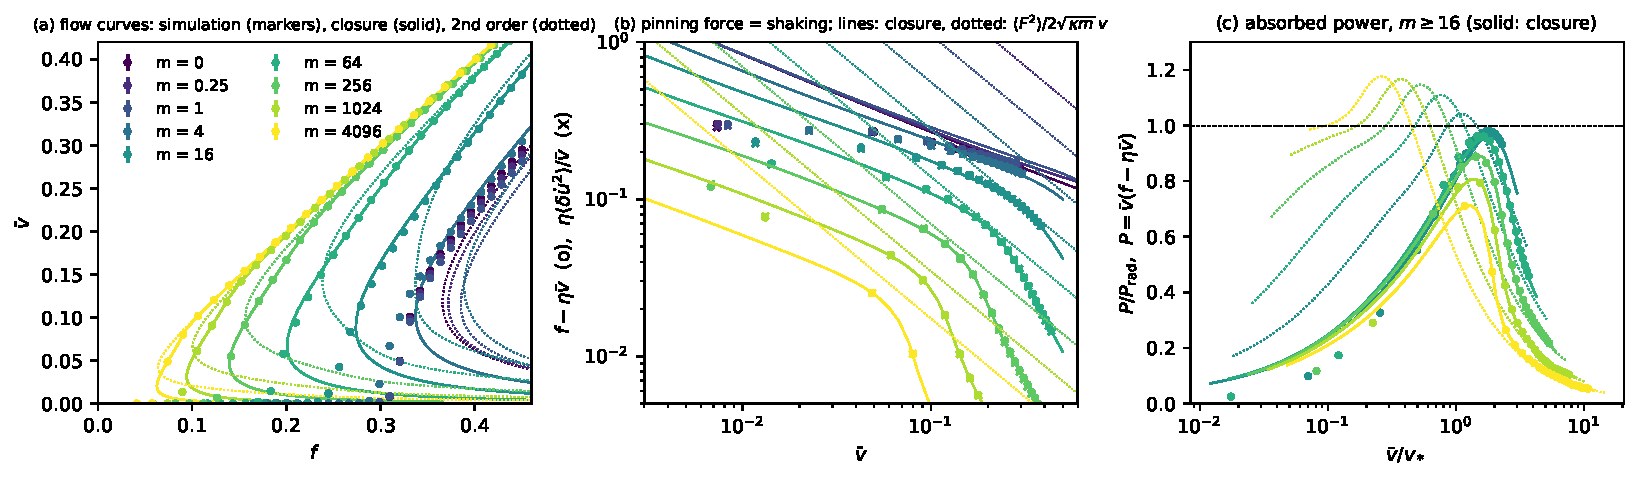
\includegraphics[width=\textwidth]{fig1_flow.pdf}
\caption{(a) Flow curves at $L=4096$: simulation (markers), hot-line closure (solid), second order (dotted). (b) Pinning force $f-\eta\bar v$ (circles) and velocity variance $\eta\langle\delta\dot u^2\rangle/\bar v$ (crosses). The two coincide, Eq.~\eqref{eq:identity}. Dotted: radiation friction $\langle F^2\rangle/2\sqrt{\kappa m}\,\bar v$. (c) Absorbed power $P=\bar v(f-\eta\bar v)$ in units of $P_{\rm rad}$ against $\bar v/v_*$, for $m\ge16$.}
\label{fig:flow}
\end{figure}

\subsection{Sliding domains below $f_{\min}$}

Just below $f_{\min}$ the line does not slide uniformly (Fig.~\ref{fig:coex}).
\begin{itemize}
\item \textbf{Domains.} Sliding domains of a few hundred sites move through a pinned line. Their edges propagate at about the sound speed $\sqrt{\kappa/m}$ ($0.031$ at $m=1024$).
\item \textbf{Sliding fraction.} The fraction $\phi$ of sites with $|\dot u_i|>0.02$ drops from 1 to 0 in a narrow window below $f_{\min}$. For $m=1024$ that window is $0.09\lesssim f\lesssim0.105$.
\item \textbf{Transient, not a phase.} These domains are how the metastable uniform state decays. Section~\ref{sec:life} shows that they do not survive at long times.
\item \textbf{Contrast with $m=0$.} Near threshold the overdamped line also shows localised activity (Fig.~\ref{fig:coex}a). Those are qEW avalanches, and they do not propagate.
\end{itemize}

\begin{figure}[H]
\centering
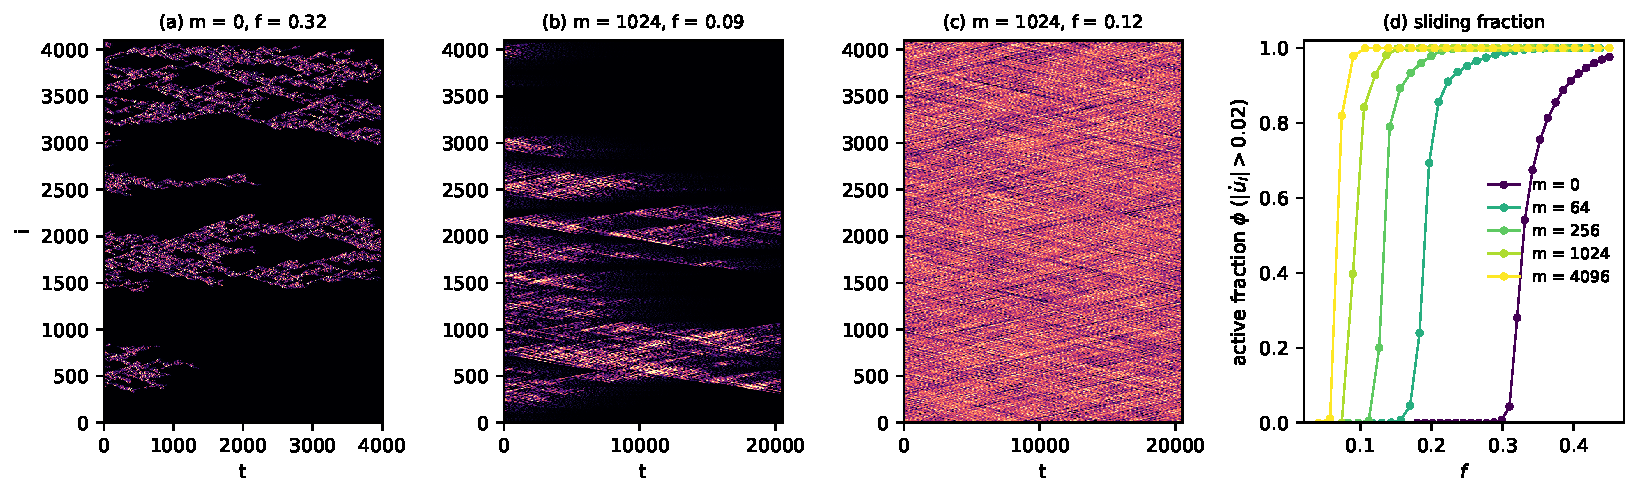
\includegraphics[width=\textwidth]{fig2_coexistence.pdf}
\caption{(a)--(c) Velocity $\dot u_i(t)$ at $L=4096$, averaged over blocks of 4 sites. (a) $m=0$ just above $\fcs$: qEW avalanches. (b) $m=1024$, $f=0.09$, below $f_{\min}=0.094$: the uniform state decaying through sliding domains, whose edges move at about the sound speed. All such lines eventually stop (Sec.~\ref{sec:life}). (c) $m=1024$, $f=0.12$: uniform hot sliding with sound waves. (d) Sliding fraction against $f$.}
\label{fig:coex}
\end{figure}

\subsection{Long-time threshold: lifetimes}
\label{sec:life}

\paragraph{Protocol.}
\begin{itemize}
\item A sliding line, prepared at $f=0.12$ ($m=1024$) or $0.17$ ($m=256$), is quenched to $f$ and run for up to $200m$.
\item It counts as stopped when its centre of mass moves less than $0.01$ in a time $m$.
\item 16 samples per point, $L=512$--4096 (Fig.~\ref{fig:life}).
\end{itemize}

\paragraph{Results.}
\begin{itemize}
\item \textbf{Below $f_{\min}$, every line stops.} At $m=1024$ ($f_{\min}=0.0943$), the median lifetime at $L=4096$ is $15m$, $18m$, $24m$, $32m$, $56m$ and $155m$ for $f=0.072$ to $0.092$. At $f=0.092$, a quarter of the lines survive the full $200m$.
\item \textbf{The lifetime diverges as $(f_{\min}-f)^{-1}$.} The fitted exponent is $1.03$ at $m=1024$ and $1.2$ at $m=256$.
\item \textbf{It barely depends on $L$.} At $f=0.088$ it is $41m$, $43m$, $47m$ and $56m$ for $L=512$ to 4096. Sliding below $f_{\min}$ is therefore not an active phase that larger systems would sustain.
\item \textbf{Above $f_{\min}$, every line keeps sliding.} At $f=0.094$, $0.096$ and $0.098$, all or nearly all lines slide for $200m$. Their mean velocities are $0.033$, $0.041$ and $0.047$, against the closure's $v_{\min}=0.030$ at $f_{\min}$.
\item \textbf{$m=256$ ($f_{\min}=0.1396$).} The switch from stopping to sliding at $L=4096$ lies between $0.132$ and $0.136$, that is $3$--$5\%$ below $f_{\min}$. Near the threshold the lifetimes still grow mildly with $L$, so this residual gap may close slowly or persist.
\end{itemize}

\paragraph{Consequence.}
The long-time stopping force is the closure minimum, $\fd(\infty)\simeq f_{\min}$, to within a few per cent and with no adjustable parameter.
The transition is discontinuous: the velocity jumps from $v_{\min}$ to zero.
The $(f_{\min}-f)^{-1}$ law is what retreating domain edges give if the edge speed vanishes linearly at $f_{\min}$.
The ramp-down value $\fd\approx0.85f_{\min}$ (Table~\ref{tab:thr}) only measures how far below $f_{\min}$ a lifetime of order the dwell time reaches.

\begin{figure}[H]
\centering
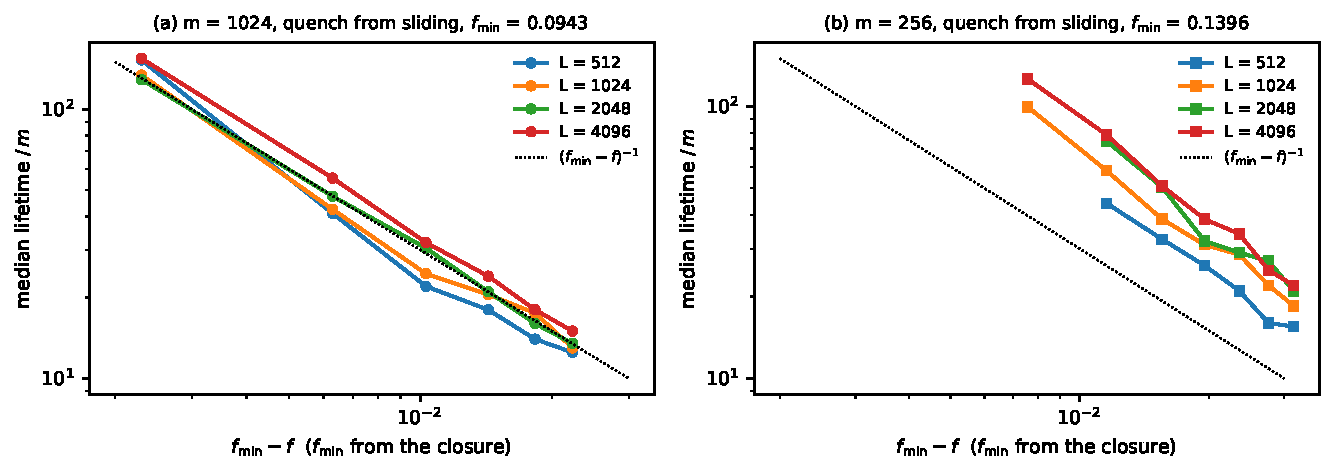
\includegraphics[width=0.85\textwidth]{fig5_lifetimes.pdf}
\caption{Median lifetime (in units of $m$) of a sliding line quenched to $f<f_{\min}$, against $f_{\min}-f$, with $f_{\min}$ from the closure. (a) $m=1024$, (b) $m=256$. Dotted: $(f_{\min}-f)^{-1}$.}
\label{fig:life}
\end{figure}

\subsection{Finite-time thresholds}

\paragraph{Protocols.}
\begin{itemize}
\item \textbf{Ramp-down.} Start sliding above threshold and lower $f$ in steps of $0.0025\,A^{4/3}$. Each step dwells for $A^{-4/3}\max(1000,10m)$. $\fd$ is the force at which the centre of mass moves less than $0.02$ over the second half of a dwell.
\item \textbf{Ramp-up.} Relax with $m=0$ at a low force, which gives a pinned state. Then raise $f$ in the same steps, each time the line is at rest ($\max|\dot u|<10^{-4}$). $\fu$ is the force at which the line travels 30 without stopping.
\item Twelve samples per point. Results are in Fig.~\ref{fig:thr} and Table~\ref{tab:thr}.
\end{itemize}

\begin{table}[H]
\centering\small
\begin{tabular}{rrcccccc}
\toprule
$m$ & $M$ & $\fd$ & $\fu$ & $f_{\min}$ (closure) & $f_*$ & $\fd/f_*$ & $\fd/f_{\min}$\\
\midrule
0 & 0 & 0.304 & 0.312 & -- & -- & -- & -- \\
1 & 0.37 & 0.301 & 0.312 & -- & 0.667 & -- & -- \\
4 & 1.5 & 0.287 & 0.298 & 0.337 & 0.471 & 0.61 & -- \\
16 & 5.9 & 0.236 & 0.253 & 0.274 & 0.333 & 0.71 & 0.86 \\
64 & 23 & 0.169 & 0.191 & 0.201 & 0.236 & 0.72 & 0.84 \\
256 & 94 & 0.118 & 0.140 & 0.140 & 0.167 & 0.71 & 0.84 \\
1024 & 376 & 0.080 & 0.107 & 0.094 & 0.118 & 0.68 & 0.85 \\
4096 & 1503 & 0.053 & 0.088 & 0.063 & 0.083 & 0.64 & 0.85 \\
\bottomrule
\end{tabular}
\caption{Finite-time thresholds for $A=1$, $L=4096$ (dwell $\max(1000,10m)$, standard errors $\le0.0015$). The static threshold is $\fcs\simeq0.308$, the mean of the $m=0$ values at $L=4096$. $f_*=(2\eta\langle F^2\rangle)^{1/2}(\kappa m)^{-1/4}$ is the second-order minimum. $f_{\min}$ is the minimum of the closure flow curve.}
\label{tab:thr}
\end{table}

\paragraph{Results.}
\begin{itemize}
\item \textbf{Ordering.} For $m\lesssim1$ ($M\lesssim0.4$) the thresholds equal $\fcs$ within $0.01$. For larger $m$, $\fd<f_{\min}$ at every size. At $L=4096$, $\fu$ lies near $f_{\min}$: slightly below for $m\le64$, where the ``travel 30'' criterion catches long transients, and above for $m\ge1024$.
\item \textbf{Ramp-down.} $\fd/f_{\min}=0.85\pm0.01$ for every $m\ge16$, at a dwell of $10m$. By Sec.~\ref{sec:life}, this ratio is set by the dwell time and the lifetime law; it is not a separate threshold.
\item \textbf{Collapse.} In reduced units $\fd/\fcs$ and $\fu/\fcs$ against $M$ fall on one curve for $A=1$ and $A=0.5$ (Fig.~\ref{fig:thr}b). $\fcs=0.308$ and $0.122$ differ by the Larkin factor $2^{4/3}$, and the closure $f_{\min}/\fcs$ collapses as well. The inertia parameter is $M$, as claimed.
\item \textbf{Size dependence.} The excess hysteresis $\Delta f=(\fu-\fd)_m-(\fu-\fd)_{m=0}$, with the $m=0$ protocol offset subtracted, shrinks roughly as $L^{-1/2}$ for $m\ge256$ (Fig.~\ref{fig:thr}c). At $m=1024$ it is $0.069$, $0.040$ and $0.020$ for $L=256$, 1024 and 4096.
\end{itemize}

\paragraph{Ramp-up nucleation.}
\begin{itemize}
\item On ramp-up the line depins once an avalanche overshoots into a hot domain that survives at that force.
\item Above $f_{\min}$ such a domain spreads, because the stretch at its edges depins the neighbours.
\item A larger line has more nucleation sites, so $\fu(L)$ falls toward $f_{\min}$. At $m=256$ and $L=4096$ it has reached it: $\fu=0.140$ against $f_{\min}=0.1396$.
\end{itemize}
In the infinite, long-time limit there is a single threshold, $f_{\min}(M)$, for both directions.
This matches the vanishing hysteresis that Schwarz and Fisher found for cellular stress-overshoot models (PRE \textbf{67}, 021603 (2003)). Here it is obtained for true inertia, and the threshold is computed.

\begin{figure}[H]
\centering
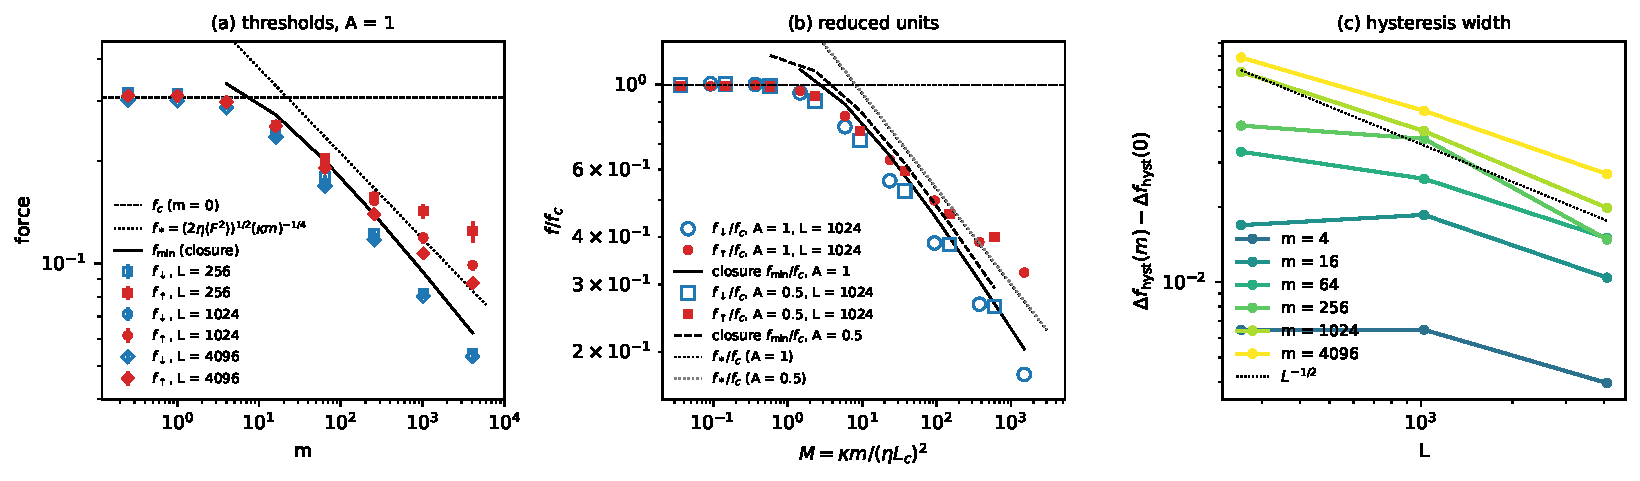
\includegraphics[width=\textwidth]{fig3_thresholds.pdf}
\caption{(a) $\fd$ (open) and $\fu$ (filled) against $m$ for $L=256,1024,4096$ ($A=1$), with $\fcs$ (dashed), the second-order scale $f_*$ (dotted) and the closure $f_{\min}$ (solid). (b) Reduced units for $A=1$ and $0.5$ at $L=1024$, against $M=\kappa m/(\eta L_c)^2$. (c) Excess hysteresis against $L$ (the $m=0$ protocol offset is subtracted).}
\label{fig:thr}
\end{figure}

\subsection{Heavy lines and random-bond disorder}

\paragraph{Runs.}
\begin{itemize}
\item Ramps at $L=1024$ for $m=16384$ and $65536$ ($M$ up to $2.4\times10^4$, $dt=1$).
\item A random-bond landscape at $m=0$--4096. Its node values are differences of i.i.d.\ values, so the potential is bounded: $\hat\Delta(k)=(A^2/3)(2-2\cos k)\,\mathrm{sinc}^4(k/2)$ and $\langle F^2\rangle=A^2/3$. The static threshold is $\fcs=0.514$.
\item The same closure, with the random-bond correlator (Fig.~\ref{fig:heavy}).
\end{itemize}

\paragraph{Debye--Waller asymptotics.}
At large $M$ the closure no longer follows $f_*\propto m^{-1/4}$. The cause is the hot line's own displacement.
\begin{itemize}
\item In the radiation regime, $P\simeq(2Z)^{-1}\int\frac{dk}{\pi}\hat\Delta(k)\,e^{-k^2B/2}$.
\item A line that has wandered $\sqrt B$ during a correlation time $r_f/v$ sees only $k\lesssim B^{-1/2}$. With $\hat\Delta(k)\propto k^{2n}$ at small $k$, this gives $P\propto B^{-a/2}/Z$ with $a=1+2n$: $a=1$ for random field, $a=3$ for random bond.
\item In the sound regime $B\simeq T(r_f/v)/Z$. With $T=mP/\eta$ and $v\simeq v_{\min}\simeq(P/\eta)^{1/2}$, this becomes $B\propto m^{1/2}P^{1/2}$.
\item Closing the loop gives $P\propto m^{-(2+a)/(4+a)}$, and therefore
\begin{equation}
f_{\min}\propto m^{-\frac{2+a}{2(4+a)}},\qquad T\propto m^{\frac{2}{4+a}}:\qquad
f_{\min}\propto\begin{cases}m^{-3/10} & \text{random field}\\ m^{-5/14} & \text{random bond}\end{cases}
\end{equation}
\item Without smearing ($a=0$) this reduces to $m^{-1/4}$.
\end{itemize}

\paragraph{Checks.}
\begin{itemize}
\item \textbf{Closure.} Its local slopes are $-0.30$ (random field, $m=4096\to16384$) and $-0.33$ (random bond, $1024\to4096$). Its temperature grows as $m^{0.43}$ for random field, against the predicted $m^{0.4}$.
\item \textbf{Random-field simulations.} The finite-time $\fd$ at $L=1024$ is $0.054$, $0.034$ and $0.021$ for $m=4096$, $16384$ and $65536$. Per factor 4 in $m$, the slopes are $-0.32$ and $-0.35$, steeper than $m^{-1/4}$.
\item \textbf{Random-bond simulations.} They give $-0.35$, against the predicted $-5/14=-0.357$.
\item \textbf{Random-bond thresholds.} They follow the random-bond closure: $\fd/f_{\min}=0.99$, $0.96$, $0.93$, $0.92$ and $0.90$ for $m=16$ to 4096, at the same dwell. Their faster fall relative to $f_*$ ($f_{\min}/f_*=0.81\to0.58$) is the $a=3$ smearing.
\end{itemize}
The disorder class therefore does enter, but only through the small-$k$ behaviour of $\hat\Delta$.
For the heaviest lines, the closure gives $f_{\min}=0.0626$, $0.0412$ and $0.0269$ at $m=4096$, $16384$ and $65536$. Its local slope settles at $-0.30$ and $-0.31$, on the random-field prediction $-3/10$.
The finite-time $\fd/f_{\min}$ falls slightly, from $0.86$ to $0.83$ and then $0.78$. That is why the simulated slope is steeper. For the heaviest lines a dwell of $10m$ is also shorter, relative to the slow sound-regime dynamics, than it is at moderate $m$.

\begin{figure}[H]
\centering
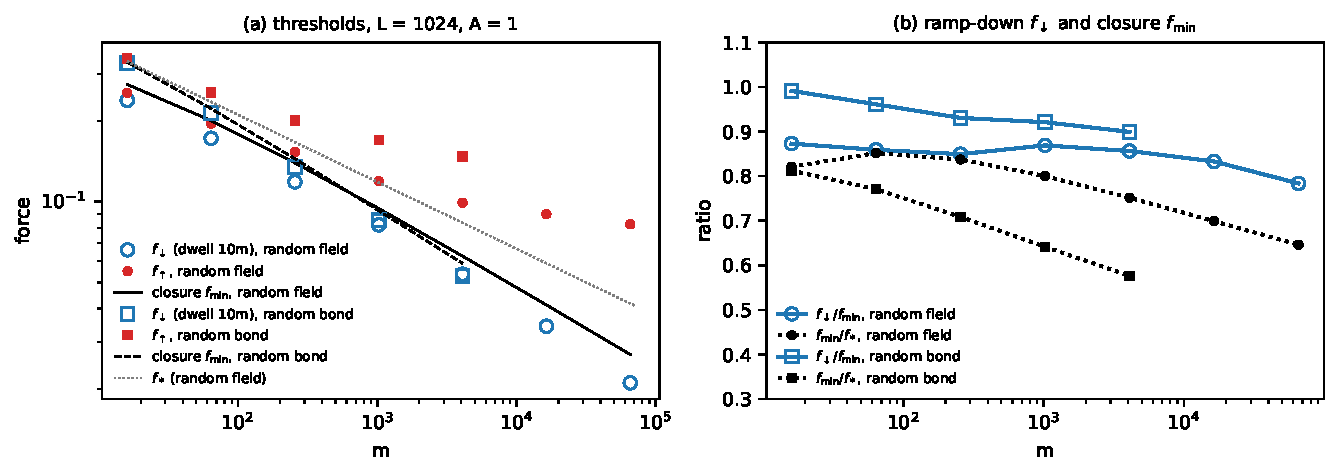
\includegraphics[width=0.85\textwidth]{fig6_heavy_rb.pdf}
\caption{(a) Finite-time thresholds at $L=1024$ for random field (circles, up to $m=65536$) and random bond (squares), with the closure $f_{\min}$ (solid: random field, dashed: random bond). (b) $\fd/f_{\min}$ (open) and $f_{\min}/f_*$ (dotted) against $m$.}
\label{fig:heavy}
\end{figure}

\subsection{Parabolic-well driving}

With a well $k_0(w-u_i)$, $k_0=0.01$, $\dot w=10^{-3}$ and $L=1024$, the force on the line is the response (Fig.~\ref{fig:well}).
\begin{itemize}
\item \textbf{$m=0$.} The force fluctuates narrowly around $0.22$. This is below $\fcs$ because the well cuts off correlations at $k_0^{-1/2}=10$ sites.
\item \textbf{$m=64$.} The mean drops to $0.165$.
\item \textbf{$m=1024$.} The motion becomes quasi-periodic stick--slip. The force is loaded up to $\approx0.12$--$0.17$, then a hot slip event unloads it to $0.05$--$0.09$. These are the finite-size ramp-up and ramp-down thresholds of a line whose correlations the well cuts off, bracketing $f_{\min}=0.094$.
\end{itemize}
Displacement driving therefore shows the hysteresis loop directly, as stick--slip around $f_{\min}$. This is the frictional face of inertial depinning.

\begin{figure}[H]
\centering
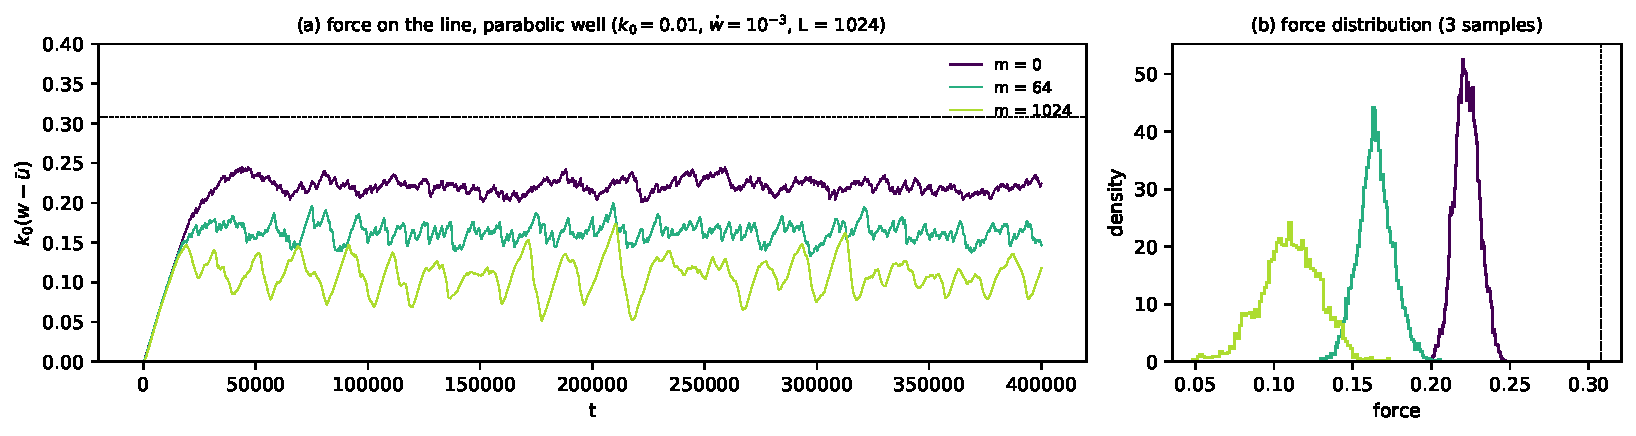
\includegraphics[width=\textwidth]{fig4_well.pdf}
\caption{(a) Force $k_0(w-\bar u)$ on the line under slow displacement driving, one sample per mass. (b) Its distribution in steady state, 3 samples. Dashed: $\fcs$ at constant force.}
\label{fig:well}
\end{figure}

\section{Summary of the theory}

\begin{center}\small
\begin{tabular}{p{2.3cm}p{6.2cm}p{6.2cm}}
\toprule
regime & thresholds & sliding state \\
\midrule
$M\lesssim1$ & $\fd\simeq\fu\simeq\fcs$ (shift $\lesssim3\%$) & qEW, continuous; inertia irrelevant ($\ell_*\lesssim L_c$) \\
$1\lesssim M\lesssim5$ & $\fcs-\fd$ grows from overshoot of single jumps & qEW-like at large scale \\
$M\gtrsim5$ & single long-time threshold $f_{\min}(M)<\fcs$ from the closure; discontinuous, velocity jump $v_{\min}$ & hot radiating string; friction $\simeq\langle F^2\rangle/2\sqrt{\kappa m}\,v$ at second order \\
$M\gg1$ & $f_{\min}\propto m^{-3/10}$ (RF), $m^{-5/14}$ (RB); $f_*\propto m^{-1/4}$ pre-asymptotic & $T\propto m^{2/(4+a)}$, Debye--Waller smearing \\
finite $L$, $t$ & decay below $f_{\min}$ in $\tau\propto(f_{\min}-f)^{-1}$; ramp-up hysteresis $\sim L^{-1/2}$ & sliding domains with sonic edges \\
\bottomrule
\end{tabular}
\end{center}

\section{Open points}

\begin{itemize}
\item \textbf{Residual gap at moderate $M$.} At $m=256$ the long-time switch lies $3$--$5\%$ below $f_{\min}$, and lifetimes near it still grow with $L$. Whether domains can survive just below $f_{\min}$ in the infinite system, as a narrow coexistence phase, needs larger $L$ and longer runs.
\item \textbf{Edge dynamics.} The $(f_{\min}-f)^{-1}$ lifetime implies hot--cold edges whose speed vanishes linearly at $f_{\min}$. A theory of such an edge, a sonic front between the closure's hot state and a pinned line, would give the prefactor and the nucleation size for ramp-up.
\item \textbf{Validity of the closure.} The Gaussian, equilibrium-shaped fluctuation spectrum is an assumption. The closure matches the sliding branch and $f_{\min}$, but a direct test of the assumed $B(\tau)$ is still missing.
\end{itemize}

\paragraph{Literature.}
\begin{itemize}
\item Schwarz and Fisher, cond-mat/0012246 (mean field) and PRE \textbf{67}, 021603 (2003): stress-overshoot automata, with mean-field tricriticality and vanishing hysteresis in large samples.
\item Maimon and Schwarz, cond-mat/0301495: one-way hysteresis.
\item de Geus and Wyart, arXiv:2204.02795 (PRE 2022) and arXiv:2411.06732: an inertial line with a non-monotonic flow curve and nucleation at $f_{\min}$, measured but not computed.
\end{itemize}
The new elements here are: the radiation friction and its scale $f_*\propto m^{-1/4}$; the parameter-free closure that computes the sliding branch and the long-time threshold $f_{\min}$; the lifetime law; the Debye--Waller asymptotics, which depend on the disorder class; and the collapse in $M$.

\paragraph{Reproduce.}
From this folder:
\begin{enumerate}
\item \texttt{python3 runs.py kymo well flow thresholds}, then \texttt{python3 runs2.py rb heavy life} and \texttt{python3 runs3.py};
\item \texttt{python3 sc\_run.py} and \texttt{python3 sc\_run2.py};
\item \texttt{python3 analyze.py} and \texttt{python3 analyze2.py}.
\end{enumerate}
The full set takes about 1.5 h on 10 cores.
\begin{itemize}
\item \texttt{sim.py}: integrator (numba, hash disorder; $A<0$ selects random bond).
\item \texttt{protocols.py}: flow, ramps, lifetimes and well protocols.
\item \texttt{linresp.py}: second-order friction.
\item \texttt{sc.py}: hot-line closure.
\end{itemize}

\end{document}
